%\documentclass[aspectratio=43]{beamer}
\documentclass[t]{beamer}
\usetheme{ffmodern}  %% Themenwahl

\usepackage[ngerman]{babel}
\usepackage[T1]{fontenc}    % richtige Silbentrennung
\usepackage[utf8]{inputenc} % Umlaute etc.!
\usepackage{eurosym}
\usepackage{tikz}
\usepackage{pgffor}
\usepackage{textcomp}
\usepackage{textpos}
\usepackage{tikz}
\usepackage{mathtools}
\usepackage{grid-system}

\usetikzlibrary{arrows,decorations.pathmorphing,backgrounds,fit,positioning,shapes.symbols,chains}

%-----------------
\title{Freifunk}
\author{Das freie WLAN-Netz} % TODO: anderer Untertitel? Bürgernetz?
\date{16. Juni 2016}
\license{CC-BY-3.0}

\begin{document}
  \maketitle

  %-----------------
  \begin{frame}{Was ist Freifunk?}
    \begin{itemize}
      \item Initiative für freie (Funk-)Netze
      \item Offen für jeden, als Nutzer oder Anbieter
      \item Netz in Nutzerhand
      \item Nicht kommerziell
      \item Netzneutral
      \item Krisensichere Kommunikation
    \end{itemize}
  \end{frame}

  %-----------------
  \begin{frame}{Was ist Freifunk?}
    \begin{center}
      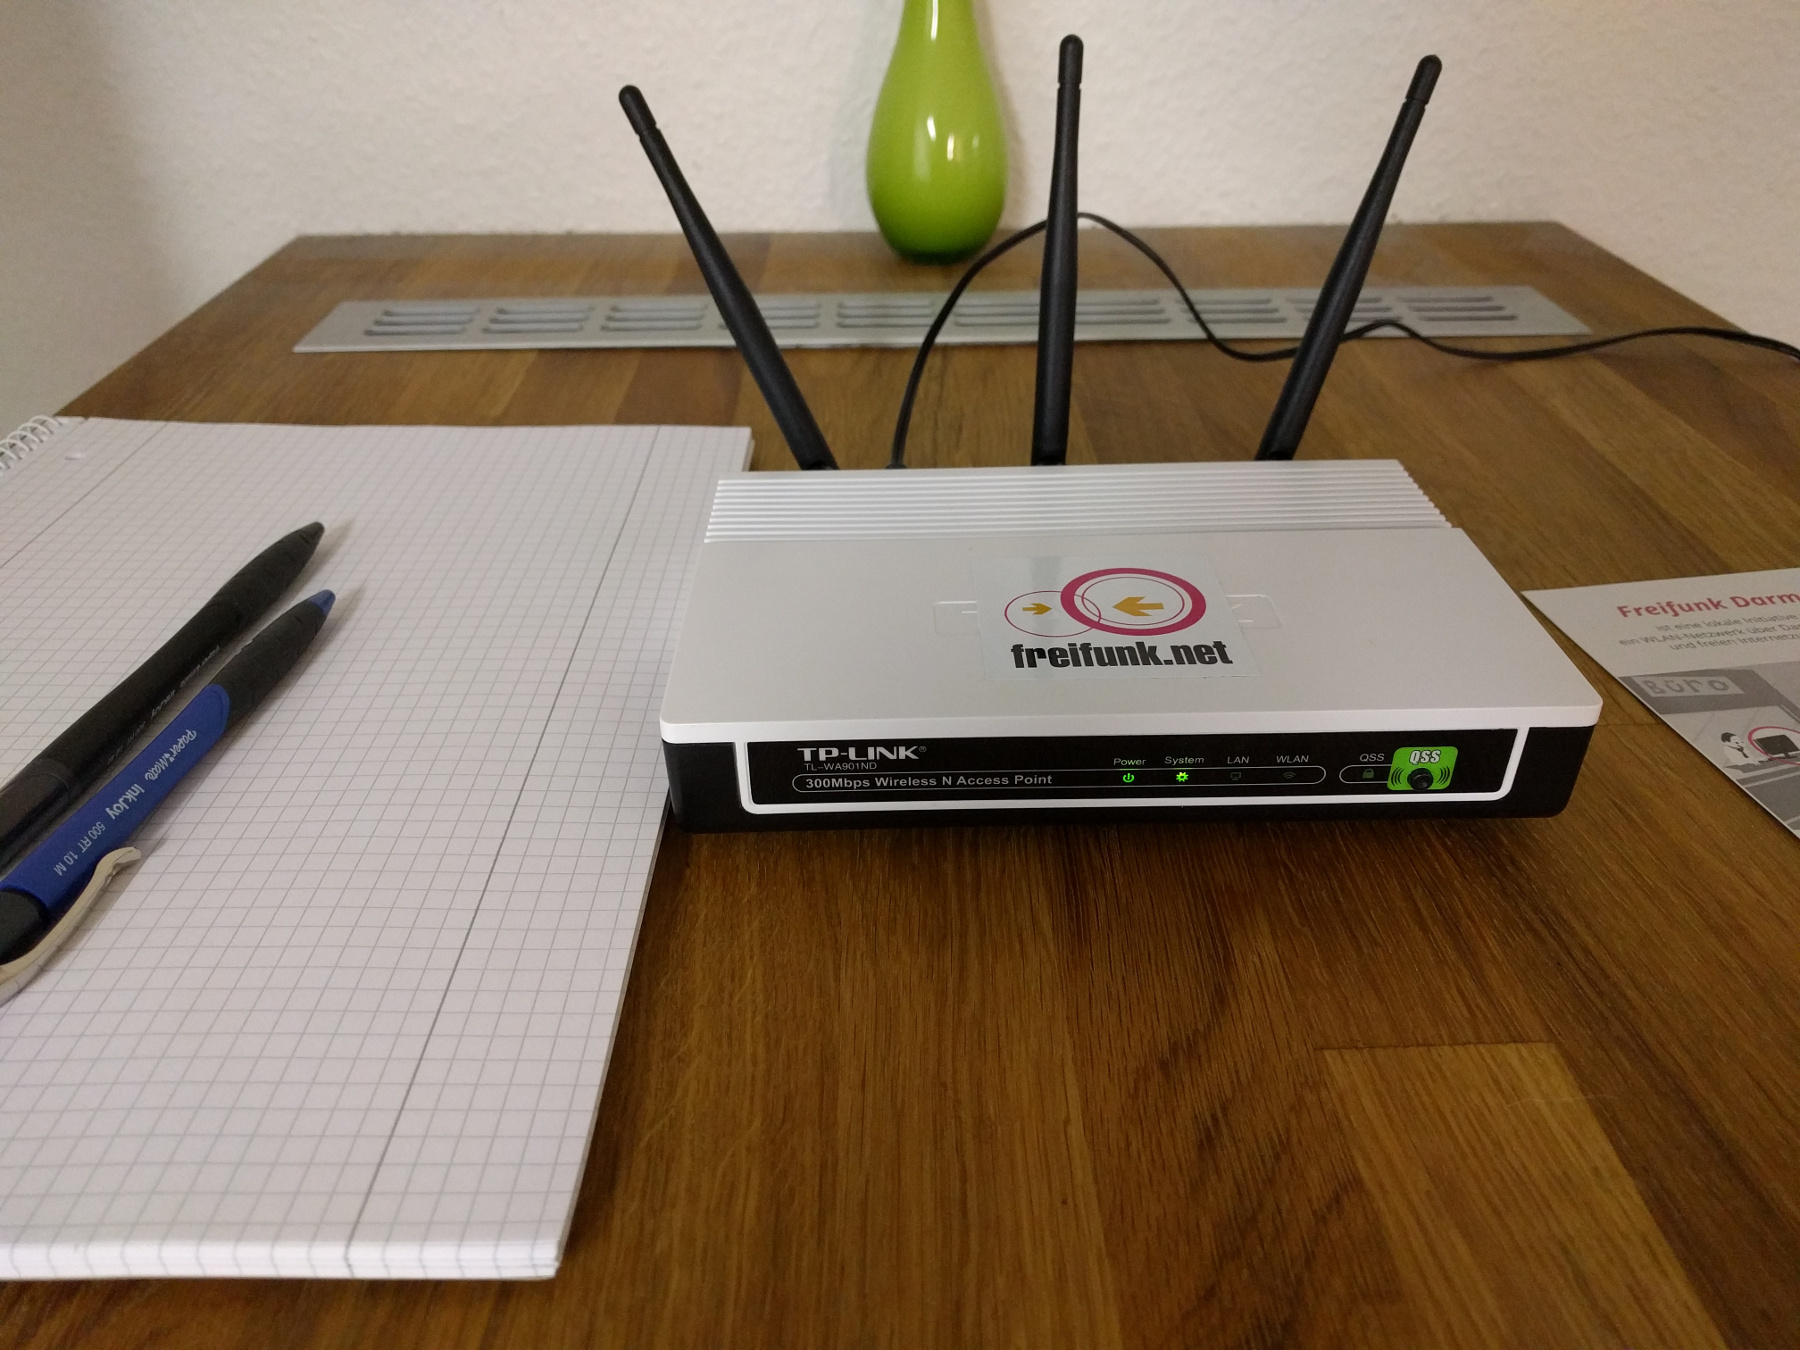
\includegraphics[width=7cm]{images/homerouter}
    \end{center}
  \end{frame}

  %-----------------
  \begin{frame}{Verbreitung}
    \begin{columns}
      \begin{column}{0.6\textwidth}
        \begin{itemize}
          \item Deutschlandweit über  \href{http://freifunk.net/wie-mache-ich-mit/community-finden/}{300 lokale Gruppen}
          \item mehr als 33.600 offene Zugangspunkte
          % TODO: Zahlen auf den aktuellen Stand bringen

        \end{itemize}
      \end{column}
      \begin{column}{0.4\textwidth}
        \begin{center}
          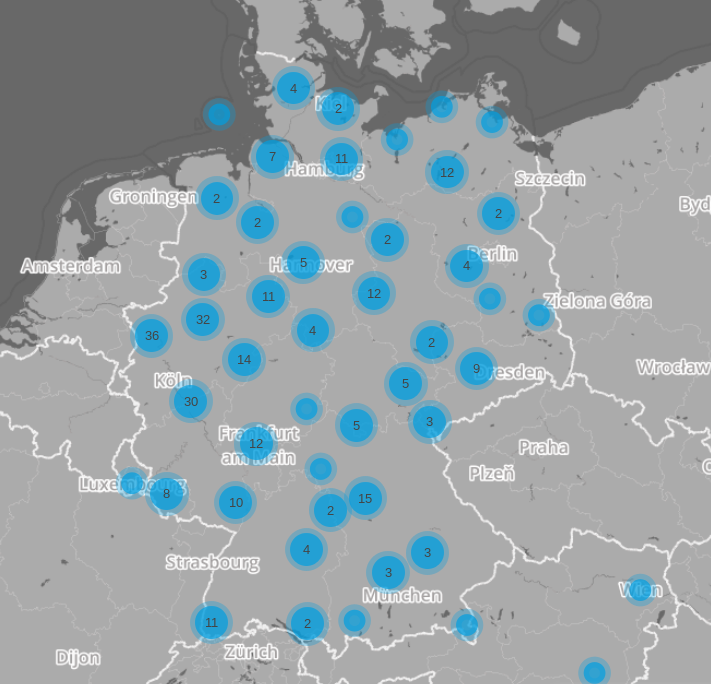
\includegraphics[width=\textwidth]{images/2016-06-01_map-de}
        \end{center}
      \end{column}
    \end{columns}
  \end{frame}

  \begin{frame}{Ziele von Freifunk}
    \begin{itemize}
      \item \textbf{Beteiligung der Bevölkerung} an Aufbau und Entwicklung \textbf{dezentraler Netze}
      \item Verständnis von Kommunikationsnetzen fördern $\xRightarrow{}$ \textbf{Bildungsauftrag}
      \item Beteilung an gesellschaftlichen Initiativen, um die \textbf{Verbreitung freier Netze} zu unterstützen
    \end{itemize}
  \end{frame}


  %-----------------
  \begin{frame}{Stadt Darmstadt}
    \begin{itemize}
      \item Über 400 Freifunk-Router in Darmstadt
      \item Täglich über 1000 Nutzer gleichzeitig online
      \item Ermöglicht durch eine starke Freifunk-Community mit großem ehrenamtlichen Einsatz
    \end{itemize}
  \end{frame}

  %-----------------
  \begin{frame}{Stadt Darmstadt}
    \begin{itemize}
      \item September 2015: Kooperation mit OB Partsch, Stadt Darmstadt vereinbart
      \item Bis Weihnachten wurden alle angefragten Unterkünfte mit WLAN versorgt
      \item Großartige Zusammenarbeit mit ASB, DRK, Feuerwehr und der städtischen IT
      \item IT Materialkosten < 5.000 \texteuro
    \end{itemize}
  \end{frame}

  %-----------------
  \begin{frame}{Stadt Babenhausen, Darmstadt-Dieburg}
    \begin{itemize}
      \item Versorgung eines Erstaufnahmelagers mit ca. 1.500 Personen in ehem. US-Kaserne
      \item Versorgung der Innenstadt entlang der Hauptachse über 1,8 km angestrebt
      \item Breitband Anbindung von Aussiedlerhöfen mit Richtfunk über bis zu 10 km
      \item Beratung des Bürgermeisters und tatkräftige Hilfe beim Aufbau einer Community
    \end{itemize}
  \end{frame}


  %-----------------
  \begin{frame}{Frankfurt am Main}
    \begin{itemize}
      \item Über 400 Freifunk-Router
      \item Täglich über 1500 Nutzer
      \item Eingetragener Verein ,,Freifunk Frankfurt e.~V.`` seit 2014
      \item Kernteam mit über 30 Experten für Entwicklung, Infrastruktur, Kommunikation
      \item Team für die Wohnsitzlosen- und Flüchtlingsarbeit mit über 20 Aktiven
    \end{itemize}
  \end{frame}

  %-----------------
  \begin{frame}{Zusammenarbeit in Frankfurt am Main}
    \begin{itemize}
      \item Empfehlungsschreiben der Stadt für alle Träger der diversen Einrichtungen
      \item Zusammenarbeit mit der Stabsstelle für Flüchtlingskoordination
      \item Enge Zusammenarbeit mit sozialen Trägern wie DRK, ASB, Johanniter, AWO, deutsch-türkische Jugendarbeit, ...
      \item Versorgung von über 20 Unterkünften mit insgesamt über 1000 Gästen
    \end{itemize}
  \end{frame}

  %-----------------
  \begin{frame}{Großraum Frankfurt am Main}
    \begin{itemize}
      \item Beratung kommunaler Mandatsträger
      \item Enge Zusammenarbeit mit Trägern und Kirchgemeinden in HTK, MTK, MKK, etc.
      \item Versorgung von ca. 12 Unterkünften mit insgesamt über 600 Gästen
    \end{itemize}
  \end{frame}

  %-----------------
  \begin{frame}{Gespräche mit Land und Kirche}
    \begin{itemize}
      \item Informationsaustausch mit der ev. Kirche Hessen-Nassau
      \item Anfragen von Kirchenvorständen, die gerne Kirchengebäude versogen würden
      \item ,,Godspot`` in Berlin-Brandenburg, daraufhin Kontakt mit Landeskirche
    \end{itemize}
  \end{frame}



  %-----------------
  %\begin{frame}{Freifunkknoten}
  %  \begin{center}
  %    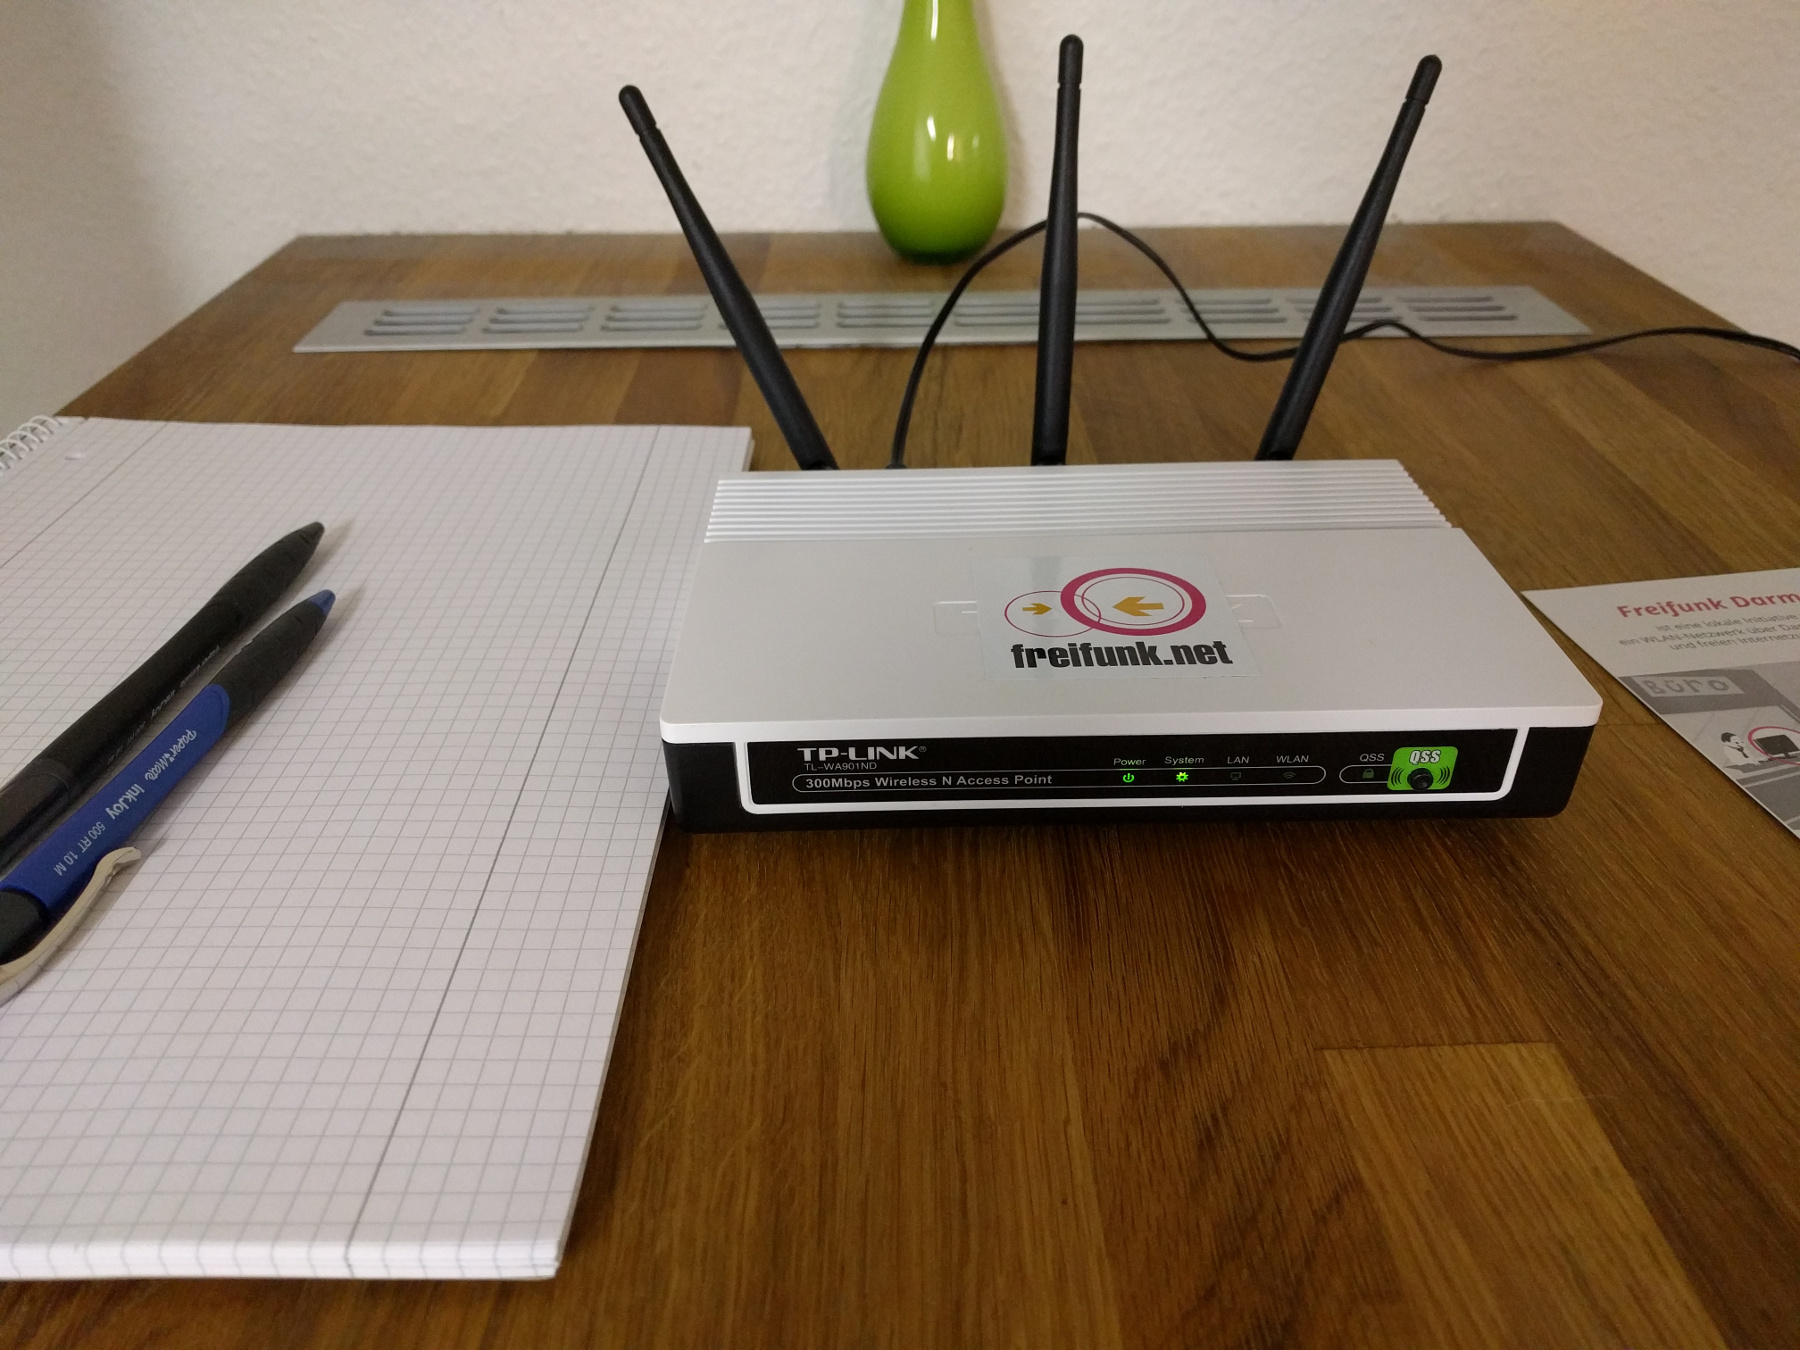
\includegraphics[width=.6\textwidth]{images/homerouter}
  %  \end{center}
  %\end{frame}
  %\foreach \index in {1, ..., 4}
  %{
  %  \begin{frame}{Das Netzwerk}
  %    \centering \includesvg[width=9cm]{netz-\index}
  %  \end{frame}
  %}

  %-----------------
  \begin{frame}{Störerhaftung}
    \begin{itemize}
      \item Keine Haftung für Knotenbetreiber
      \item Internetverkehr geht über unsere Gateways. Haftungsbefreiung nach TMG \S8.
      \item Wir nehmen die gesetzlichen Vorschriften wörtlich: Wir sammeln keine Daten.
    \end{itemize}
  \end{frame}

  %-----------------
  \begin{frame}{Richtfunknetz}
    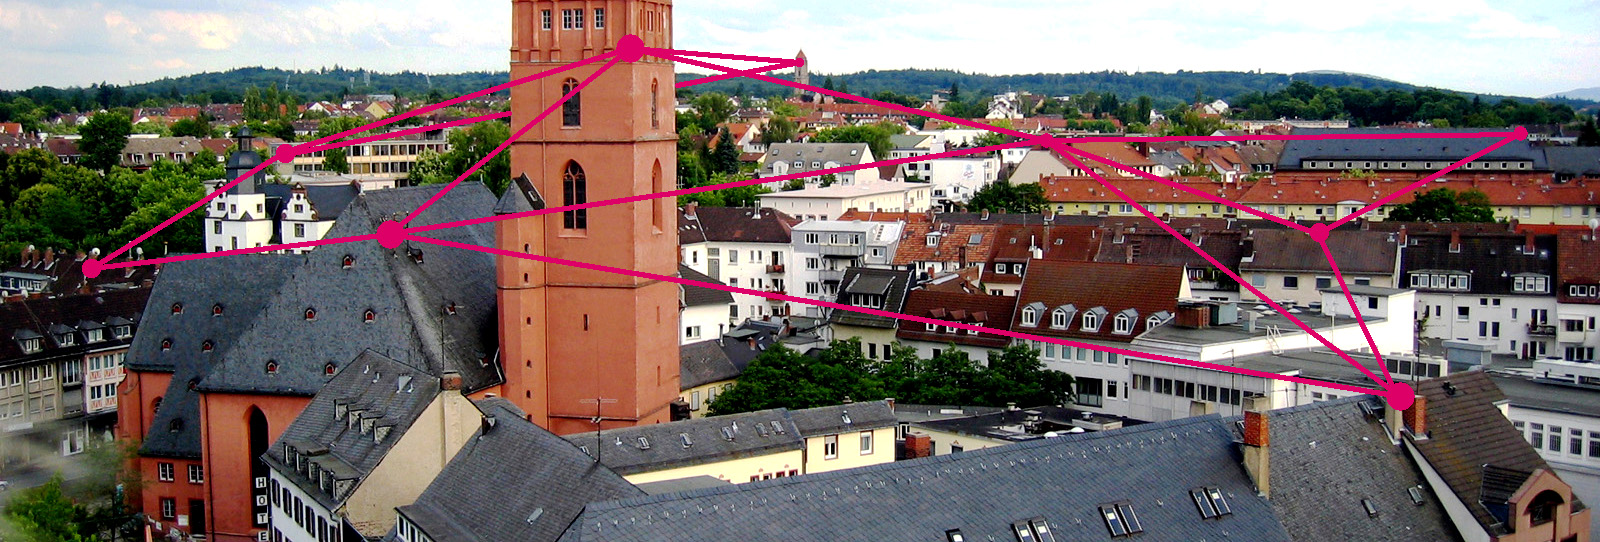
\includegraphics[width=\textwidth]{images/banner-stadtkirche-darmstadt}
    \begin{columns}
      \begin{column}{0.65\textwidth}
        \begin{itemize}
          \item Eigene Infrastruktur
          \begin{itemize}
            \item Redundanz und Lastverteilung
            \item Unabhängig vom Internet
          \end{itemize}
        \end{itemize}
      \end{column}
      \begin{column}{0.25\textwidth}
        \begin{center}
          \vspace{-1.5cm}
          \hspace{-0.75cm}
          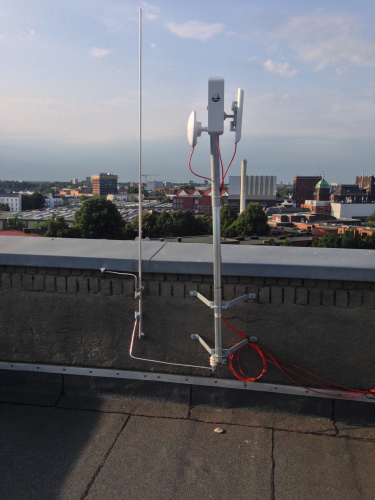
\includegraphics[width=\textwidth]{images/hamburg-richtfunkmast}
        \end{center}
      \end{column}
    \end{columns}
  \end{frame}

  %-----------------
  \begin{frame}{Richtfunknetz}
    \begin{center}
      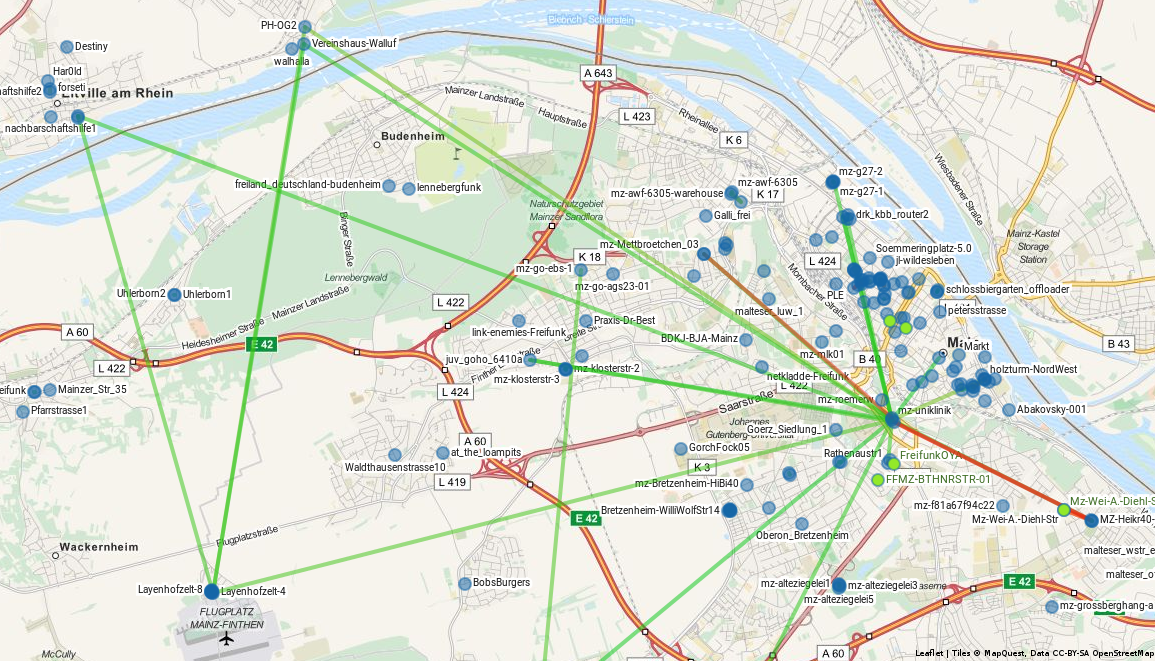
\includegraphics[width=0.95\textwidth]{images/2016-06-12_map-mainz-rifu}
    \end{center}
  \end{frame}

  %-----------------
  \begin{frame}{Freifunk lebt vom Mitmachen}
    \begin{itemize}
      \item Freifunk ist \textbf{kein Dienstleister}
      \item Aufbau einer \textbf{lokalen Community} (falls nicht vorhanden) wünschenswert
      \item Andere Freifunk-Gruppen helfen gerne dabei und \textbf{geben Wissen weiter}
    \end{itemize}
  \end{frame}

  %-----------------
  \begin{frame}{Kosten}
    \begin{itemize}
      \item Internetzugang durch Freifunker (Privatpersonen, Träger, Kommunen)
      \item Hardware je nach Nutzungsart ab 15,- €
      \item Kosten für Infrastruktur: Ca. 6,- \texteuro\ pro Router und Jahr
    \end{itemize}
  \end{frame}

  %-----------------

  \begin{frame}{Vielen Dank!}
    \begin{textblock*}{0cm}(\textwidth-2cm,-2cm)
      \begin{figure}[h]
        \def\svgwidth{2.5cm}
        \input{logo.pdf_tex}
      \end{figure}
    \end{textblock*}
    \begin{itemize}
      \item Freifunk Frankfurt
      \begin{itemize}
        \item Webseite: \href{http://wifi-frankfurt.de}{wifi-frankfurt.de}
        \item E-Mail: info@wifi-frankfurt.de
        \item Treffen: Jeden ersten Montag und Sonntag im Monat
      \end{itemize}
      \item Freifunk Darmstadt
      \begin{itemize}
        \item Webseite: \href{http://darmstadt.freifunk.net/}{darmstadt.freifunk.net}
        \item E-Mail: info@darmstadt.freifunk.net
        \item Treffen: Jeden Montag um 18:30 Uhr
      \end{itemize}
      \vspace{1em}
      \item Liste aller Communities auf \href{https://freifunk.net/}{freifunk.net}
    \end{itemize}
  \end{frame}
\end{document}
